%% Use the option review to obtain double line spacing
\documentclass[authoryear,preprint,review,12pt]{elsarticle}

%% The amssymb package provides various useful mathematical symbols
\usepackage{amssymb}
%% The amsthm package provides extended theorem environments
%% \usepackage{amsthm}
%% The xcolor package provides colored text
\usepackage{xcolor}
%% The listings package provides a way to include code in an article
\usepackage{listings}
\definecolor{mygray}{rgb}{0.8,0.8,0.8}
\lstset{
  basicstyle=\ttfamily,
  backgroundcolor=\color{mygray}
}
%% this allows us to add inline code with a gray background
\newcommand{\code}[1]{\colorbox{mygray}{\vphantom{Tg}\lstinline|#1|}}
%% this adds hrefs to citations
\usepackage[colorlinks,citecolor=red,urlcolor=blue,bookmarks=false,hypertexnames=true]{hyperref} 
%% so i dont need to add path every time
\graphicspath{ {./graphics/} }
%% remove "preprint submitted to elsevier" from template
\makeatletter
\def\ps@pprintTitle{%
 \let\@oddhead\@empty
 \let\@evenhead\@empty
 \def\@oddfoot{}%
 \let\@evenfoot\@oddfoot}
\makeatother

\begin{document}

\begin{frontmatter}

  %% Title, authors and addresses

  %% use the tnoteref command within \title for footnotes;
  %% use the tnotetext command for theassociated footnote;
  %% use the fnref command within \author or \affiliation for footnotes;
  %% use the fntext command for theassociated footnote;
  %% use the corref command within \author for corresponding author footnotes;
  %% use the cortext command for theassociated footnote;
  %% use the ead command for the email address,
  %% and the form \ead[url] for the home page:
  %% \title{Title\tnoteref{label1}}
  %% \tnotetext[label1]{}
  %% \author{Name\corref{cor1}\fnref{label2}}
  %% \ead{email address}
  %% \ead[url]{home page}
  %% \fntext[label2]{}
  %% \cortext[cor1]{}
  %% \affiliation{organization={},
  %%            addressline={}, 
  %%            city={},
  %%            postcode={}, 
  %%            state={},
  %%            country={}}
  %% \fntext[label3]{}

  \title{\textbf{G}itHub \textbf{O}nline \textbf{A}nalytics}

  %% use optional labels to link authors explicitly to addresses:
  %% \author[label1,label2]{}
  %% \affiliation[label1]{organization={},
  %%             addressline={},
  %%             city={},
  %%             postcode={},
  %%             state={},
  %%             country={}}
  %%
  %% \affiliation[label2]{organization={},
  %%             addressline={},
  %%             city={},
  %%             postcode={},
  %%             state={},
  %%             country={}}

  \author[inst1]{Moritz Fuller}

  \affiliation[inst1]{organization={Humboldt Universitaet zu
        Berlin},%Department and Organization
    addressline={Unter den Linden 6},
    city={Berlin},
    postcode={10117},
    state={Berlin},
    country={Germany}}

  \begin{abstract}
    \textbf{GOA} (GitHub Online Analytics) is a web application that provides
    a graphical overview of the evolution of a GitHub repository.
  \end{abstract}

  %%Graphical abstract
  % \begin{graphicalabstract}
  %   
\includegraphics{grabs}
  % \end{graphicalabstract}

  %%Research highlights
  % \begin{highlights}
  %   \item Research highlight 1
  %   \item Research highlight 2
  % \end{highlights}

  % \begin{keyword}
  %   %% keywords here, in the form: keyword \sep keyword
  %   keyword one \sep keyword two
  %   %% PACS codes here, in the form: \PACS code \sep code
  %   \PACS 0000 \sep 1111
  %   %% MSC codes here, in the form: \MSC code \sep code
  %   %% or \MSC[2008] code \sep code (2000 is the default)
  %   \MSC 0000 \sep 1111
  % \end{keyword}

\end{frontmatter}

%% \linenumbers

\section{Motivation of research problem and research question}
\label{sec:motivation}

There are many tools to analyze GitHub repository data, but from a first shallow research each of
them comes with certain drawbacks. You either need to install something, configure a complicated
setup, pay for it, the use case is too specific or it's focussing more on data around the git
protocol itself rather than the social part of GitHub . What's missing is a lightweight, flexible
and easy to use GitHub Online Analytics (GOA) tool.

The question we are trying to answer in our thesis is what kind of tools are out there, how do they
function and what kind of features do they provide. We want to achieve this by developing a
framework to compare each one of the services using certain criteria that are being explained in
more detail in section \ref{sec:method}. Using this comparison we can identify a niche, an ideal
product that does not exist yet and that we are going to develop then.

The next step would be to find out what kind of data should be visualized and how it should be
visualized. We will try to use the ESeVis framework developed by
\citet{yeshchenkoSurveyApproachesEvent2022} to categorize the visualization techniques used by
current solutions, although it seems to focus on event sequence data, which is not our primary
focus for this tool. At the same time we want develop a framework that categorizes the different
data points that are available for analysis. We might settle on the "Common Metrics" defined by
\citet{CHAOSSCommonMetrics2022}.

For now the plan is to develop a webapp allowing you to enter the link for a GitHub repository you
want to analyze. The webapp will then make calls to the GitHub GraphQL API to retrieve the data and
visualize it using a framework like d3.js, Vega-Lite or ECharts. Ideally the user should be able to
configure the data being analyzed and how it's visualized using a simple interface.

\section{Summary of background literature and state of the art solutions}
\label{sec:summary}

There are numerous tools out there that can be used to analyze GitHub repositories. In the
following chapters we will give a quick overview of the ones that are closest to what we are trying
to achieve and outline their characteristics.

\subsection{Apache Kibble}
\label{sec:summary:kibble}

Apache Kibble is a suite of tools for collecting, aggregating and visualizing activity in software
projects developed by the Apache Software Foundation. It has to be deployed manually and can be
configured to scan multiple different data sources like GitHub, JIRA or a mailing list. It has no
releases, but users can try the development version. The project seems abandoned as the last commit
to main as of writing this was 13 months ago. The configuration and setup are non trivial and
require a good knowledge of the underlying technologies like UNIX, Python and Apache HTTP Server
\citep{ApacheKibble2022}.

\subsection{Augur}
\label{sec:summary:augur}

Augur is a Python library and web service for Open Source Software Health and Sustainability
metrics \& data collection. It has to be deployed manually and can be configured to scan multiple
different data sources like GitHub, git commit logs and the Core Infrastructure Initiatives API. It
is actively maintained and while there a Docker images available for a quick deployment, when used
for long-term data collection it still requires nontrivial installation steps. Those include
setting up a PostgreSQL database, installing the instance, an application server and Augur's data
collection workers \citep{Augur2022}.

\subsection{Gitinspector}
\label{sec:summary:gitinspector}

Gitinspector is a statistical analysis tool for git repositories. It can be installed locally using
npm or a package manager like apt-get and provides a command line utility. Python and git need to
be present on the system, together with the repository that should be analyzed. It focuses on a
single repository and enables users to compare distinct contributors. It is mainly used as a
grading aid by universities. Although the project has 2.1k stars on GitHub, it seems abandoned, as
the last commit was 2 years ago \citep{EjwaGitinspector2022}.

\subsection{Frontend Repo Analyzer}
\label{sec:summary:repoanalyzer}

The Frontend Repo Analyzer is a tool that can analyze git repositories and report metrics about
them. It supports multiple repositories and can be configured for a variety of metrics. As the name
suggests it focuses more on repositories that contain Frontend code, it does read the dependencies
from a \code{package.json} file. or the CSS bundle size for example. The installation is quite
easy, as it's available for npm, but there is still some setup left to do for the data base which
stores the results after each run and the configuration of the tool. The project seems to be
maintained \citep{FrontendRepoAnalyzer2022}.

\subsection{Grimoire Lab}
\label{sec:summary:grimoire}

Grimoire Lab provides a coordinated set of tools to retrieve data from systems used to support
software development (repositories), store it in databases, enrich it by computing relevant metrics
and making it easy to run analytics and visualizations on it. Although they provide a docker image
to ease start playing, if used in a production environment extensive configuration and setup of
each one of the tools is required. For an overview see Figure \ref{fig:grimoire-overview}. It is
actively maintained and there are multiple projects building on this stack, like Cauldron
\ref{sec:summary:cauldron} and Insights \ref{sec:summary:insights}
\citep{duenasGrimoireLabToolsetSoftware2021,GrimoireLab2022}.

\begin{figure}[h]
  \centering
  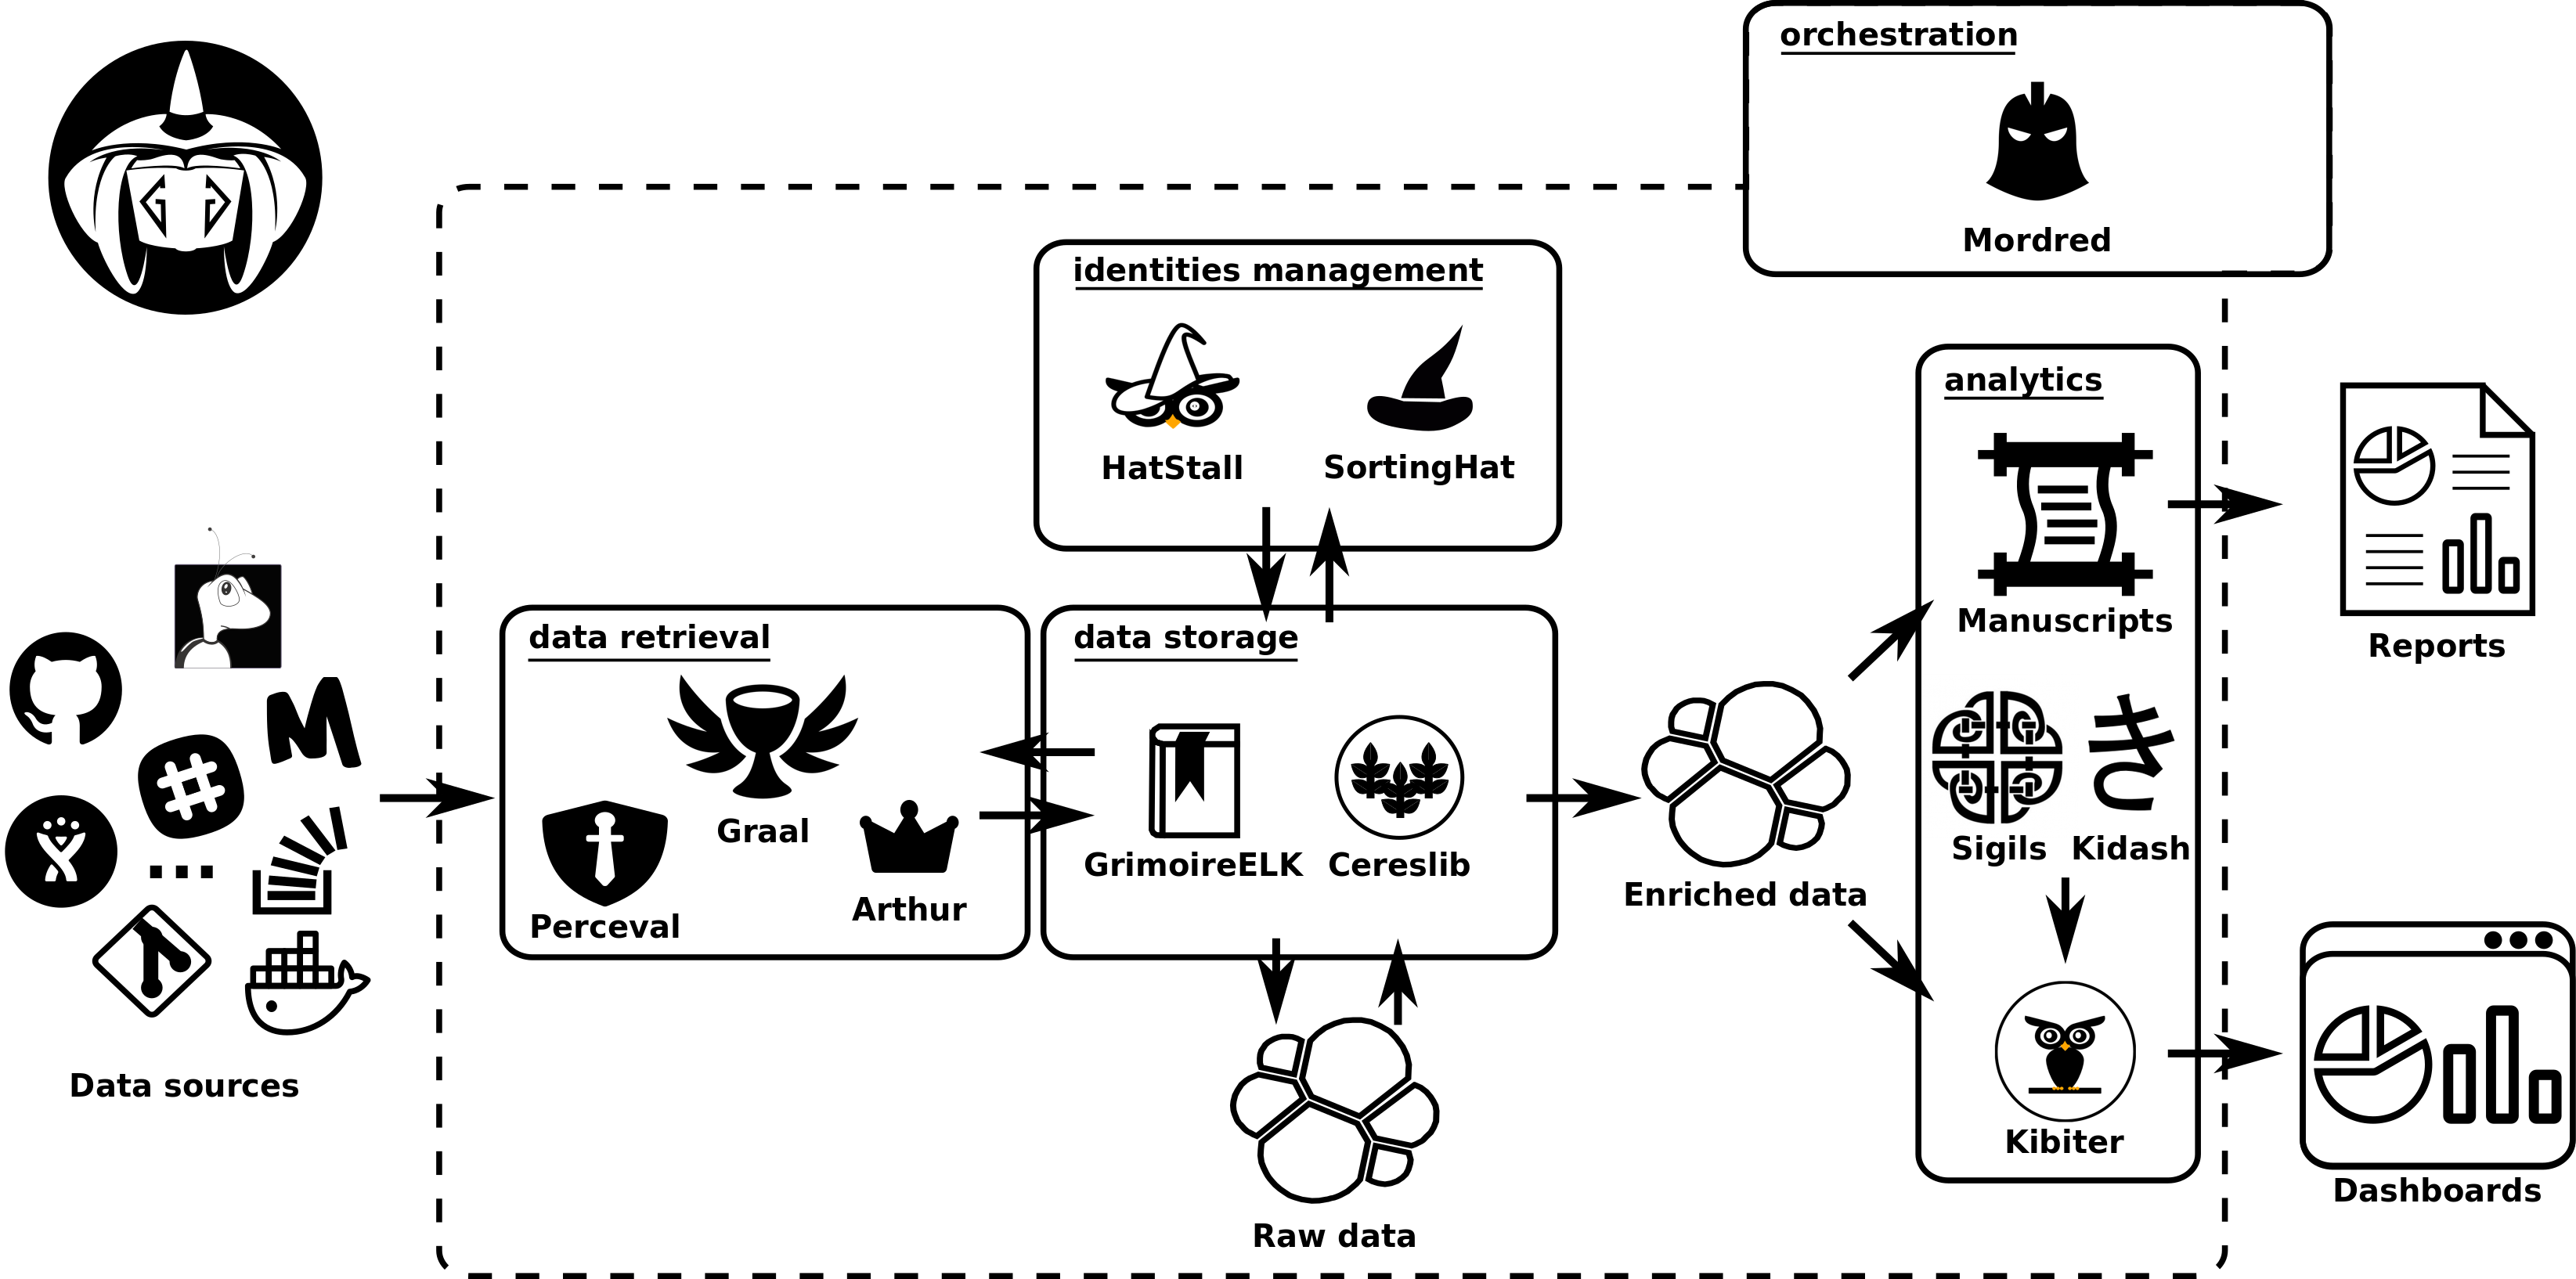
\includegraphics[width=\linewidth]{graphics/grimoirelab-all-details}
  \caption{Grimoire Lab tool stack \citep{GrimoireLab2022}}
  \label{fig:grimoire-overview}
\end{figure}

\subsection{Haystack}
\label{sec:summary:haystack}

Haystack is a tool to provide insights from Git data, to help experiment faster, ship reliably and
prevent burnout. So far it is the tool that seems to come the closest to what we are trying to
achieve apart from the difference that it's closed source and a paid service. Users only need to
create an Haystack account, connect their version control system and choose which repositories to
plug into Haystack. It's not entirely clear what the dashboard provides, as there is no accessible
demo available \citep{HaystackAnalyticsEngineering}.

\subsection{LFX Insights}
\label{sec:summary:insights}

LFX Insights provides data-driven insights to make informed decisions. It follows the best
practices and specifications from the CHAOSS project, with some of the components being initially
sourced from Grimoire Labs. Users are able to connect multiple data sources like emails, GitHub,
Google Groups or Twitter to a project. There is no obvious self hosting available and enrolling on
their instance your own project requires you to create an account to submit a ticket for onboarding
\citep{Insights}.

\subsection{Cauldron}
\label{sec:summary:cauldron}

Cauldron is another project that builds on the Grimoire Lab stack. It is a web application that
allows users to create so called reports that contain a set of repositories from multiple data
sources. Cauldron then collects and analyzes the data to display it in a dashboard. Reports created
with Cauldron are persisted and visible for everyone. It's possible to setup your own paid instance
of Cauldron via Cauldron Cloud \citep{CauldronCloud} or to deploy the project yourself. The
dashboard contains a variety of graphs and analytics out of the box and can be further customized
and extended using the Elastic dashboard tied to every project. Apart from that it's possible to
compare different projects. Cauldron seems to be maintained, but rather irregular. It's another
tool that is very close to what we are trying to achieve.
\citep{CauldronCauldron,LevelSoftwareDevelopment}.

\subsection{Monocle}
\label{sec:summary:monocle}

Monocle enables users to organize daily duties and to detect anomalies in the way changes are
produced and reviewed. They provide a docker deployment got get started quickly, but they also
document deploying from source. When deploying a \code{config.yaml} file has to be present, which –
among other things – specifies the repositories to be analyzed. It comes with a sensible set of
default visualizations that are configurable. Monocle is actively developed \citep{Monocle2022}.

\subsection{RepoSense}
\label{sec:summary:reposense}

RepoSense is a tool to visualize programmer activities across git repositories. You can either use
it locally – which requires Java and git – or remotely using a service like Netlify or GitHub
Actions to generate so called reports. A report consists of an interactive website and can be
viewed using a browser. The reports can be customized to a degree using CLI flags and config files,
but visualization is rather rigid. The project is actively maintained \citep{RepoSense2022}.

\begin{figure}[h]
  \centering
  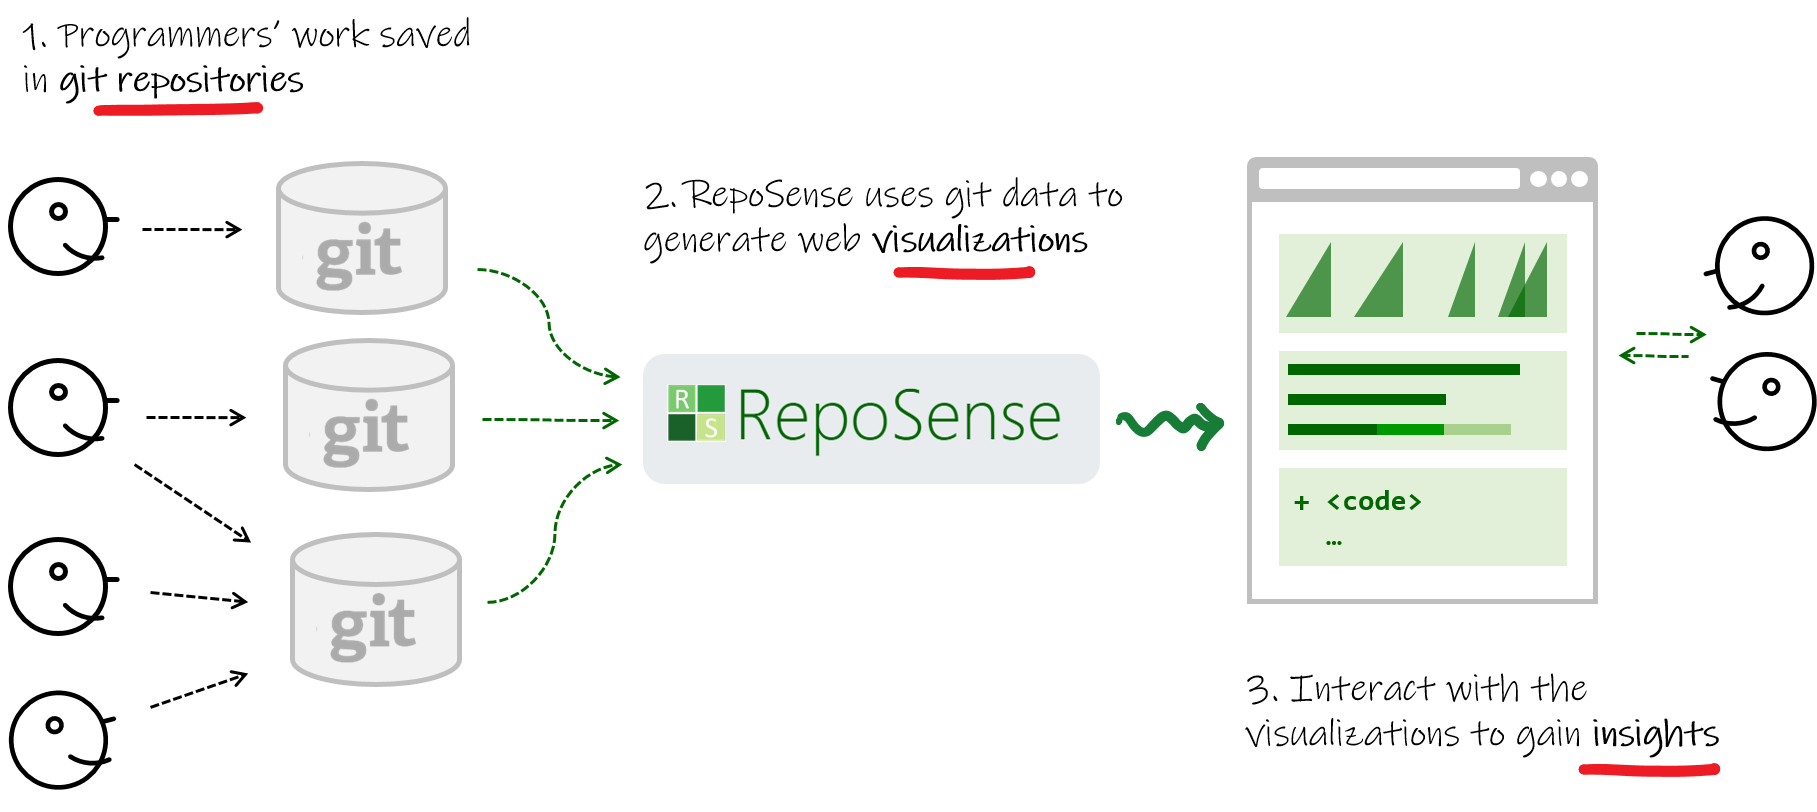
\includegraphics[width=\linewidth]{reposenseOverview}
  \caption{RepoSense overview \citep{RepoSenseHome}}
  \label{fig:reposense}
\end{figure}

\section{Proposed research method}
\label{sec:method}

First we want to analyze the current landscape of available tools and compare them in terms of
functionality, events processed and visualization techniques.

\subsection{Functionality}
The following properties are used to compare the functionality of the tools:

\subsubsection{hosted}
This property describes wether the tool is hosted or requires deployment.

\subsubsection{maintained}
This property describes wether a tool is actively maintained or not. To be considered actively
maintained there have to be at least 5 commits to the release branch within the past 6 months.

\subsubsection{difficulty}
The difficulty is described using the following categorization:
\begin{itemize}
  \item easy : no installation, no setup, plug \& play
  \item medium : requires some setup, but easy to use (e.g download a package or run a docker image)
  \item hard: requires setting up databases, servers, configurations and use of the CLI
\end{itemize}

\subsubsection{comparisons}
This characteristic describes wether the tool allows to compare at least two different repositories
with one another.

\subsubsection{customizable / explorable}
We evaluate wether the tool is customizable in some way. This means that the user can configure
different metrics and visualizations with low effort and visually explore the data.

\subsubsection{open source}
We evaluate wether or not the projects source code is open source to allow community contributions
and further enhancements.

\subsubsection{repository focused}
We evaluate wether the tool is focused on single repositories or on general data.

\subsubsection{free}
We evaluate wether the tool is free or requires a paid license.

\subsubsection{database}
Does the tool make us of it's own database to store the data or rely on a third party database.

\subsection{Metrics}
We will most likely use the "Common Metrics" provided by \citet{CHAOSSCommonMetrics2022} to compare
the different tools out there. The working group focuses on defining metrics that are used by
multiple working groups or are important for community health. The focus areas of those metrics
are:
\begin{itemize}
  \item contributions
  \item people
  \item place
  \item time
\end{itemize}

\subsection{Visualization}
We could analyze existing solutions regarding the visualizations they are using, although we are
not sure yet how useful this would be for our goals. Nevertheless the following properties could be
used:
\begin{itemize}
  \item scatter plot
  \item theme river
  \item bar chart
  \item area chart
  \item line chart
  \item heatmap
  \item stacked bar chart
  \item pie chart
  \item bubble chart
  \item tree map
  \item radar chart
  \item ESeViz charts \citep{yeshchenkoSurveyApproachesEvent2022}
\end{itemize}

\section{Outline of thesis}
\label{sec:outline}

%% make nested enumerate numbers instead of letters
\renewcommand{\labelenumii}{\arabic{enumi}.\arabic{enumii}}
\renewcommand{\labelenumiii}{\arabic{enumi}.\arabic{enumii}.\arabic{enumiii}}
\renewcommand{\labelenumiv}{\arabic{enumi}.\arabic{enumii}.\arabic{enumiii}.\arabic{enumiv}}

\begin{enumerate}
  \item Introduction
        \begin{enumerate}
          \item Background
          \item Terminology
          \item Research Question
          \item Structure
        \end{enumerate}
  \item Evaluating state of the art solutions
        \begin{enumerate}
          \item Functionality
          \item Metrics
          \item (Visualization)
          \item The "perfect" tool
        \end{enumerate}
  \item Technologies
        \begin{enumerate}
          \item Svelte
          \item Tailwind
          \item d3 $\mid$ ECharts $\mid$ Vega-Lite
          \item Apollo Svelte
        \end{enumerate}
  \item Artifact
  \item Conclusion
\end{enumerate}

\section{Preliminary literature list}
\label{sec:literature}

See \ref{sec:bibliography} for the complete list.

\section{Work plan including milestones}
\label{sec:workplan}
\begin{table}[h]
  \centering\begin{tabular}{ |c | c| }
    \hline
    due date & task                               \\
    \hline
    15.05.22 & finish evaluation                  \\
    \hline
    18.05.22 & identify niche and specify product \\
    \hline
    25.05.22 & specify technologies               \\
    \hline
    01.07.22 & produce artifact                   \\
    \hline
    01.08.22 & submit thesis                      \\
    \hline
  \end{tabular}
  \caption{Work plan}
  \label{fig:workplan}
\end{table}
%% create a list of figures & tables
\listoffigures
\listoftables

%% add all items from the bib file to the references
\nocite{*}
\bibliographystyle{elsarticle-harv}
\bibliography{cas-refs}
\label{sec:bibliography}

\end{document}

\endinput